\section{Grafiskt användargränssnitt}
Beskrivning för installation och användande av GUI:t till QuadOpt.

\subsection{Installation}
För att kunna använda QuadOpt via det grafiska användargränssnittet så behöver endast Python vXXX eller senare vara installerad.

\subsection{Användning}
\begin{enumerate}
	\item Packa upp \emph{quadopt.zip} i en valfri mapp.
	\item Öppna en kommandotolk i samma mapp.
	\item Starta programmet genom att skriva \textbf{python GUI.py}. Om du använder Windows och detta inte skulle fungera, så kan det bero på att du inte har sökvägen till Python inlagt i \emph{Environment variables}. Skriv då istället sökvägen till där du har Python installerat innan anropet. Exempelvis \textbf{C:/Python33/python GUI.py}
	\item Nu visas ett fönster enligt figur 1. 
	\item Klart! QuadOpt är nu installerat i Matlab och är redo att köras.
\end{enumerate}

\begin{figure}[h]
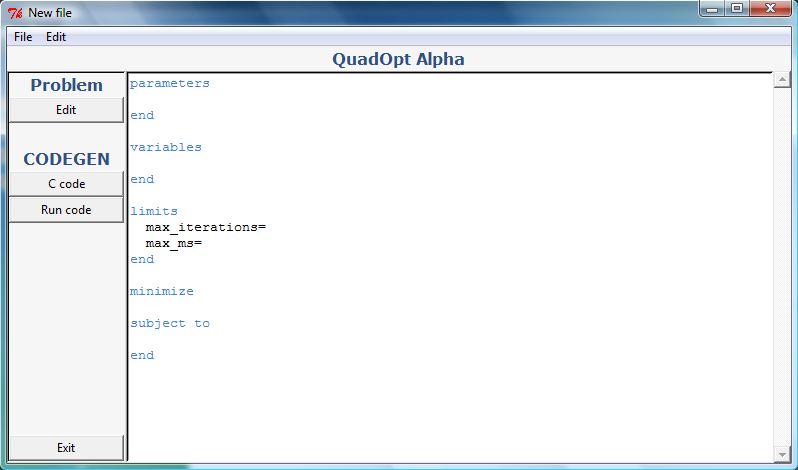
\includegraphics[scale=0.52]{bilder/gui.png}
\caption{Det grafiska gränssnittet.}
\end{figure}